
\chapter{Introducción}\label{cap:intro}

El triaje es un proceso que clasifica a los pacientes según su nivel de gravedad o el riesgo de desarrollar una condición determinada. Cuando se aplica en una sala de internación general \cite{bancomundial_enfermeras_parteras}, ayuda a mejorar la calidad de la atención en comparación con los métodos tradicionales, contribuyendo a reducir la mortalidad inesperada al aumentar la frecuencia de los controles de enfermería en los pacientes más graves y disminuirla en aquellos menos graves \cite{liao2020novel,lee2018systematic}.

Aunque el triaje se puede realizar manualmente, este método está sujeto a errores y puede incrementar la carga de trabajo del personal de salud. En un sistema de historia clínica digital, se presenta la oportunidad de integrar el triaje en la plataforma. Sin embargo, los sistemas convencionales, cuyo enfoque principal es la documentación, pueden no ser adecuados para implementar de manera efectiva una solución que, a partir de los resultados del triaje, guíe el proceso de atención de los pacientes en sus diversos aspectos. Incluso si fuera posible, la solución carecería de portabilidad hacia otros sistemas de historia clínica digital. Por lo tanto, una opción más viable es desarrollar una aplicación específica e independiente, capaz de interoperar con cualquier sistema de historia clínica digital y otros sistemas de salud, lo que facilita su adopción por diversas instituciones.

La herramienta propuesta, denominada ALERTAR \cite{latorre2024alertar}, está diseñada para la vigilancia y la emisión de alertas tempranas en unidades de cuidados no intensivos, centrando su atención en el paciente y su condición clínica. ALERTAR optimiza el proceso de vigilancia de enfermería mediante la generación de alertas visuales y sonoras en dispositivos móviles, advirtiendo al personal de la proximidad o el retraso de los controles programados. Estos intervalos de control se establecen en función del nivel de riesgo calculado mediante un algoritmo de triaje, que se basa en los datos clínicos de los pacientes ingresados.

El sistema tiene un diseño orientado a la recopilación de datos históricos de los pacientes, lo cual da lugar a la mejora del algoritmo de triaje a lo largo de su tiempo de vida, además de permitir el acceso a estos datos históricos desde cualquier dispositivo móvil de una manera rápida y sencilla para el usuario.

Esta funcionalidad se representa en la Figura \ref{fig:transformacionDatos} donde se observa la transformación de los datos. Esto abarca el ingreso de datos clínicos de un paciente, el resultado del cálculo del nivel de riesgo, y el cálculo del horario del siguiente control de enfermería en función del nivel de riesgo obtenido. A su vez, se observan alertas, que el sistema genera en función de los diferentes datos. Estas alertas son avisos que informan sobre las situaciones que podrían requerir una acción. Estas pueden comunicarse de dos maneras: como alarmas y como notificaciones. Las alarmas buscan captar atención inmediata mientras que las notificaciones son informativas y menos intrusivas.

La aplicación determina el nivel de gravedad de los pacientes (bajo, moderado, alto y crítico), utilizando el algoritmo de triaje y se encarga de alertar al personal de salud (médicos y enfermeros) de dichos cambios. Además, según el nuevo nivel de riesgo calculado, se configuran automáticamente próximos controles de enfermería para el paciente. Este control se notifica al enfermero responsable de la tarea cuando le corresponda realizarlo, incluyendo alertas en caso de retrasos. Esto permite al personal de la salud incrementar su rendimiento, reduciendo los controles a pacientes estables y priorizando la asistencia a aquellos en condiciones graves. El personal de la salud, además de recibir estas notificaciones en sus dispositivos móviles, con el objetivo de evaluar la evolución del paciente, cuentan con un registro electrónico simplificado de datos clínicos específico para la enfermedad tratada.

\begin{figure}
    \centering
    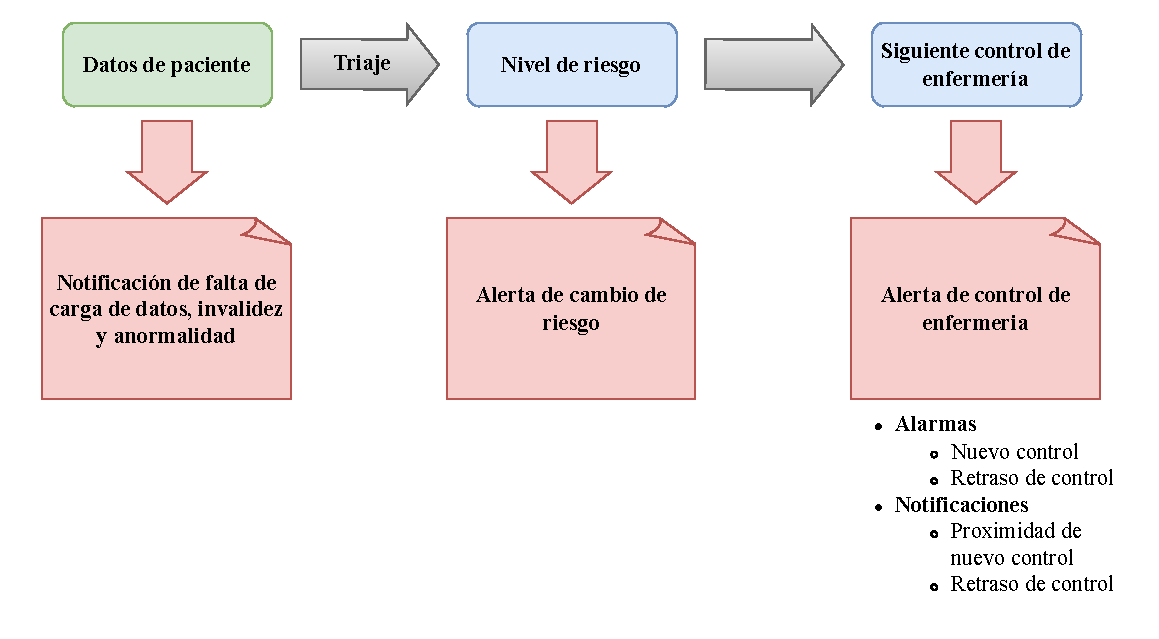
\includegraphics[width=\linewidth]{Imagenes/Intro/TransformacionDatos.pdf}
    \caption{Ingreso y transformación de los datos}
    \label{fig:transformacionDatos}
\end{figure}
El objetivo de ALERTAR es operar en una gran cantidad de hospitales. Por esto, se diseñó para garantizar su funcionamiento incluso en condiciones de conectividad limitada, adaptándose tanto a variaciones en la calidad de la conexión a Internet como a diferencias en la infraestructura de red dentro de cada sector hospitalario. Dado que se trata de un sistema crítico para la atención de pacientes, se requiere un alto grado de resiliencia. Para cumplir con este requisito, el sistema debe garantizar la comunicación entre dispositivos a través de una red de área local (LAN). Esto permite que los dispositivos sigan comunicándose y sincronizándose, asegurando el funcionamiento local del sistema aún en caso de pérdida de conexión a Internet.

Los siguientes requerimientos del sistema influyen directamente en la elección de la solución técnica: 
\begin{enumerate}
    \item Uso exclusivo de dispositivos móviles en lugar de infraestructura adicional como computadoras o servidores locales. Esto facilita la adopción y despliegue del sistema, especialmente en hospitales con recursos limitados.
    \item El sistema debe mantenerse operativo y confiable, es decir ser resiliente, ante fallos en la infraestructura de red, problemas de hardware o software. Esto es crucial debido a la importancia de garantizar la continuidad del servicio en la atención de pacientes.
    \item El alcance del sistema debe ser multi hospitalario, para permitir la recolección masiva de datos clínicos, lo cual es esencial para la calibración continua de los sistemas de alerta temprana y el incremento de la capacidad predictiva del sistema.
\end{enumerate}

Ante estos desafíos, el sistema ALERTAR fue diseñado con una arquitectura distribuida que optimiza la resiliencia frente a fallos de conectividad y hardware. La metodología adoptada en su desarrollo permite garantizar su operatividad en entornos hospitalarios con condiciones variables de red.
% Agregar solucion global
% Se propone una arquitectura distribuida en nube, niebla y borde... a partir de esto enlazo con objetivos

%Redefinir objetivos especificos cosa que coincida con lo que hice.

\section{Objetivos y alcance de la tesis}
El objetivo general de esta tesis es:

\begin{center}
    \textit{Implementar un prototipo básico del núcleo de la aplicación móvil del sistema ALERTAR.} 
\end{center}

Se considera que el núcleo de la aplicación móvil comprende toda la funcionalidad de la aplicación con excepción de la interfaz gráfica. En esta tesis se desarrolla un prototipo básico del núcleo de la aplicación móvil, compuesto por una plataforma base y un conjunto limitado de casos de uso implementados sobre ella.

La experimentación sobre este prototipo permite validar la plataforma base, e identificar posibles mejoras arquitectónicas o de implementación, con el fin de establecer una base sólida que permita completar, en etapas posteriores, la funcionalidad prevista para el dominio de la aplicación móvil.
\\\\
Para alcanzar el objetivo general se definen los siguientes objetivos específicos:
\begin{enumerate}
    \item Implementar la capa de transporte de datos de la aplicación móvil, permitiendo:
    \begin{itemize}
        \item Comunicaciones seguras, que garanticen la protección de información confidencial de pacientes. 
        \item Monitorear la conectividad de la aplicación móvil con otros componentes del sistema (dispositivos móviles y la nube) para detectar la interrupción de conexiones.
    \end{itemize}
        

    \item Implementar el mecanismo de tolerancia a fallos de la aplicación móvil basado en replicación de datos entre dispositivos móviles y la nube.

    \item Verificar el correcto funcionamiento del mecanismo de tolerancia a fallos mediante una validación funcional con casos de uso básicos del dominio, incluyendo pruebas de concurrencia.
    
    \item Realizar una evaluación del rendimiento de la aplicación móvil implementada, considerando:
    \begin{itemize}
        \item Eficiencia del almacenamiento local de datos.
        \item Tiempo de ejecución de operaciones básicas del mecanismo de tolerancia a fallos basado en replicación de datos.
    \end{itemize}

    
\end{enumerate}

%Objetivos especificos:
%- Implementar un mecanismo de toleracia a fallos basado en la replicacion de datos considerando los siguientes aspectos calve...

%- Implementar un protocolo de comunicaciones destinado a interconectar los diversos componentes que integran al sistema ALERTAR, de manera tal que se logre...

%- Relizar un marco teorico el cual sustente las decisiones de diseño y tecnologicas adoptadas.

%- Explorar como la integracion de dispositivos moviles como infraestructura hospitalaria, facilitan la gestion y aseguran la resiliencia en entornos medicos criticos

%- Explorar como la integracion del sistema ALERTAR con una arquitectura cloud-fog-edge contribuye a la eficiencia del sistema y a la mejora de la atencion medica, proporcionando una infraestructura resiliente, escalable y segura

\section{Metodología}
ALERTAR es la evolución del sistema COVINDEX \cite{chiarotto2024covindex, chiarottoJornadasCloud}, desarrollado durante la pandemia de COVID-19. Debido al contexto de urgencia sanitaria, COVINDEX fue implementado de manera apresurada y experimental, sin un diseño previo detallado, sin visión a futuro y con limitaciones en cuanto a escalabilidad, lo que lo restringe únicamente al tratamiento de casos de COVID-19.

Ante la necesidad de un sistema más generalizado, surgió la oportunidad de diseñar un sistema que asista a médicos y enfermeros en unidades de cuidados intensivos, sin limitarse a una sola patología. A partir de esta necesidad, se desarrolló el diseño arquitectónico y se establecieron los lineamientos básicos para implementar un sistema más amplio. Este trabajo de tesis se encarga del desarrollo de un prototipo básico del núcleo de la aplicación móvil del sistema ALERTAR a partir de dicho diseño.

El desarrollo del sistema ALERTAR se estructura en tres componentes principales: implementación del servidor remoto (nube), diseño e implementación de la interfaz gráfica móvil, y diseño e implementación del núcleo de la aplicación móvil, siendo el prototipo básico de este último el foco de este trabajo de tesis. El proyecto se llevó a cabo de manera colaborativa entre profesores y alumnos. En paralelo, un profesor estuvo a cargo de la implementación del componente de la nube, mientras que tres alumnos se dedicaron al desarrollo de la interfaz gráfica móvil. Esta colaboración facilitó considerablemente tanto el desarrollo como la prueba del núcleo de la aplicación móvil, permitiendo la validación y puesta en marcha de la aplicación directamente en dispositivos móviles llegando a tener a día de hoy un prototipo funcional.

\section{Trabajos relacionados}
Una aplicación que trabaja sobre el mismo dominio y tiene objetivos similares a ALERTAR es Intramed \cite{intraMed}. Intramed es una plataforma que monitorea a los pacientes dentro de un hospital, permitiendo almacenar y acceder a información clínica de los mismos. Utiliza una segunda aplicación llamada Vitals360 \cite{Vitals360} para monitorear en tiempo real los signos vitales de los pacientes. En conjunto, ambas proporcionan resultados intuitivos y sencillos para los usuarios en forma de listas y gráficos, permitiendo llevar a cabo expedientes electrónicos de los pacientes. Además, Intramed registra información relativa a médicos, enfermeros, documentos clínicos, reservas de quirófanos o laboratorios y facilita la comunicación entre profesionales a través de la escritura.

Si bien los dispositivos de Intramed, cuando pierden conexión con Internet, almacenan localmente la información y la envían una vez restablecida la conexión, estos no pueden compartir información entre sí por más que se encuentren en un mismo hospital donde podrían aprovechar, por ejemplo, la red de área local (LAN). Esto es malo dado que existe riesgo de pérdida de los datos ante fallos de dispositivos móviles y tiene impacto directo en la atención al paciente debido a la incapacidad de compartir información crucial de manera rápida y eficiente, lo que afecta al monitoreo apropiado de los pacientes. En cambio, ALERTAR cuenta con un sistema de comunicación auxiliar por red de área local para evitar la desconexión en zonas con acceso débil o nulo a Internet. Esta propiedad es vital para ofrecer un servicio crítico en la atención de pacientes.

Otra aplicación relacionada es eWeLink \cite{eWeLink}, la cual se utiliza para controlar dispositivos inteligentes para el hogar, especialmente aquellos basados en tecnología de Internet de las cosas. La aplicación permite a los usuarios controlar y monitorear dispositivos del hogar inteligente a través de dispositivos móviles, permitiendo encender o apagar luces, electrodomésticos y otros dispositivos desde cualquier lugar con conexión a Internet. eWeLink realiza una comunicación entre dispositivos similar a la de ALERTAR, ya que funciona tanto a través de Internet como por medio de una red LAN. Sin embargo, trabaja en un contexto y dominio totalmente diferente y el nivel de resiliencia es bajo debido a que la funcionalidad se ve notablemente reducida cuando no se cuenta con acceso a la red de Internet.

Por último, COVINDEX \cite{chiarotto2024covindex, chiarottoJornadasCloud} es la versión antecesora de ALERTAR, su objetivo es monitorear pacientes con COVID-19 y proporcionar alertas tempranas de gravedad. Debido al contexto de emergencia, se implementó rápidamente sin un diseño extensible, limitando su aplicación exclusivamente al COVID-19, quedando como un prototipo experimental.
%Agregar comparativa


\section{Organización del resto del trabajo}
En el capítulo \ref{cap:marcoTeorico}, se presenta el marco teórico de los elementos y fundamentos que sustentan el desarrollo del prototipo básico del núcleo de la aplicación móvil del sistema ALERTAR. En el capítulo \ref{cap:arquitecturaGeneral}, se detalla la arquitectura general del sistema, explicando los componentes que la conforman. El capítulo \ref{cap:implementacion} aborda la implementación de la aplicación móvil. En el capítulo \ref{cap:experimentacion}, se presentan los resultados de los experimentos realizados. Finalmente, en el capítulo \ref{cap:conclusionesYTrabajosFuturos}, se exponen las conclusiones derivadas del desarrollo del prototipo básico del núcleo de la aplicación móvil del sistema ALERTAR y se enumeran posibles trabajos futuros a realizar.